\documentclass[reqno]{amsart}
\usepackage[utf8]{inputenc}
\usepackage[margin=1in]{geometry}
\usepackage[usenames, dvipsnames]{xcolor}
\usepackage{graphicx}
\usepackage{mathtools}
\usepackage{amssymb}
\usepackage{amsthm}
\usepackage{fancyhdr}
\usepackage{adforn}
\usepackage{xparse}
\usepackage{tikz}
\usetikzlibrary{fadings}
%\usetikzlibrary{matrix, positioning, calc}
% Additional math macros that I want in both my notes and my psets
\usepackage[sc, noBBpl]{mathpazo}
\usepackage{mathrsfs}
\usepackage[T1]{fontenc}
\usepackage{calligra}
\usepackage{microtype}
\usepackage[all]{xy}
\usepackage{slashed}
\newcommand{\A}{\mathbb A}
\newcommand{\cat}{\mathsf}
\newcommand{\sC}{\cat C}
\newcommand{\sD}{\cat D}
\newcommand{\sS}{\cat S}
\newcommand{\sA}{\mathscr A}
\newcommand{\sF}{\mathscr F}
\newcommand{\sG}{\mathscr G}
\renewcommand{\P}{\mathbb P}
\newcommand{\cO}{\mathscr O}
\newcommand{\sI}{\mathscr I}
\DeclareMathOperator{\coker}{coker}
\renewcommand{\Im}{\operatorname{Im}}
\newcommand{\pt}{\mathrm{pt}}
\DeclareMathOperator{\Hom}{Hom}
\newcommand{\op}{^{\mathsf{op}}}
\newcommand{\Id}{\mathrm{Id}}
\DeclareMathOperator{\Mat}{Mat}
\newcommand{\m}{\mathfrak m}
%\newcommand{\p}{\mathfrak p}
\newcommand{\q}{\mathfrak q}
\DeclareMathOperator{\MSpec}{MSpec}
\DeclareMathOperator{\Spec}{Spec}
\newcommand{\Top}{\cat{Top}}
\newcommand{\Ring}{\cat{Ring}}
\newcommand{\Mod}{\cat{Mod}}
\DeclareMathOperator{\res}{res}
\newcommand{\Alg}{\cat{Alg}}
\newcommand{\Fun}{\cat{Fun}}
\newcommand{\AffSch}{\cat{AffSch}}
\newcommand{\Ab}{\cat{Ab}}
\DeclareMathOperator{\bl}{--}
\DeclareMathOperator{\Free}{Free}
\DeclareMathOperator{\For}{For}
\newcommand{\Set}{\cat{Set}}
\newcommand{\LocRing}{\cat{LocRing}}
\newcommand{\Grp}{\cat{Grp}}
\newcommand{\Sch}{\cat{Sch}}
\newcommand{\inHom}{\operatorname{\underline{\Hom}}}
\DeclareMathOperator{\Frac}{Frac}
\DeclareMathOperator{\Gal}{Gal}
\DeclareMathOperator{\Nil}{Nil}
\newcommand{\pre}{\sC^{\text{pre}}}
\newcommand{\sh}{_{\text{sh}}}
\newcommand{\G}{\mathbb G}
\DeclareMathOperator{\Proj}{Proj}
\newcommand{\sM}{\mathscr M}
\newcommand{\sV}{\mathscr V}
\newcommand{\fU}{\mathfrak U}
\newcommand{\GL}{\mathrm{GL}}
\DeclareMathOperator{\Sym}{Sym}
% http://tex.stackexchange.com/questions/141434/how-to-type-sheaf-hom
\DeclareMathOperator{\shom}{\mathscr{H}\text{\kern -4pt {\calligra\large om}}\,}
\newcommand{\sL}{\mathscr L}
\DeclareMathOperator{\QC}{QC}
\DeclareMathOperator{\Supp}{Supp}
\newcommand{\sN}{\mathscr N}
\DeclareMathOperator{\Ann}{Ann}
\DeclareMathOperator{\Der}{Der}
\newcommand{\ctcpx}[1]{(#1)^{\text{der}}}
\newcommand{\Dist}{\mathsf{Dist}}
\newcommand{\shdi}{\operatorname{Sh}_{\Dist}}
\DeclareMathOperator{\Sh}{Sh}
\newcommand{\shz}{\mathsf{Sh}_{\text{\rm Zar}}}
\DeclareMathOperator{\Gr}{Gr}
% Source: http://tug.org/pipermail/xy-pic/2001-July/000015.html
\newcommand{\pullbackcorner}[1][dr]{\save*!/#1+1.2pc/#1:(1,-1)@^{|-}\restore}
\newcommand{\pushoutcorner}[1][dr]{\save*!/#1-1.2pc/#1:(-1,1)@^{|-}\restore}
\newcommand{\TDel}{\mathrm{2\Delta}}
\DeclareMathOperator{\Bl}{B\ell}
\newcommand{\cR}{\mathcal R}
\newcommand{\cL}{\mathcal L}
\newcommand{\cH}{\mathcal H}
\newcommand{\refR}{\reflectbox{\(\cR\)}}

\renewcommand{\a}{\alpha}
\renewcommand{\b}{\beta}
%\newcommand{\e}{\epsilon}
\renewcommand{\l}{\lambda}
\renewcommand{\L}{\Lambda}
\newcommand{\g}{\gamma}
\newcommand{\s}{\sigma}
\newcommand{\z}{\zeta}
\newcommand{\RR}{\mathbb{R}}
\newcommand{\NN}{\mathbb{N}}
\newcommand{\QQ}{\mathbb{Q}}
\newcommand{\ZZ}{\mathbb{Z}}
\newcommand{\CC}{\mathbb{C}}
\newcommand{\cC}{\mathcal{C}}
\newcommand{\f}{\frac}
\newcommand{\p}{\partial}
\renewcommand{\P}[3][]{\f{\partial^{#1} #2}{\partial #3 ^{#1}}}
%\newcommand{\avg}[1]{\langle #1 \rangle}
\newcommand{\avg}[1]{\left< #1 \right>}
\newcommand{\?}{\overset{?}{=}}
\newcommand{\Int}{\int_{-\infty}^\infty}
\newcommand{\ket}[1]{\left| #1 \right>} % for Dirac bras
\newcommand{\bra}[1]{\left< #1 \right|} % for Dirac kets
\newcommand{\braket}[2]{\left< #1 \vphantom{#2} \right|
 \left. #2 \vphantom{#1} \right>} % for Dirac brackets
\newcommand{\pv}{\vec{p}}

\newcommand{\grad}[1]{\gv{\nabla} #1} % for gradient
\let\divsymb=\div % rename builtin command \div to \divsymb
\renewcommand{\div}[1]{\gv{\nabla} \cdot #1} % for divergence
\newcommand{\curl}[1]{\gv{\nabla} \times #1} % for curl
\renewcommand{\labelenumi}{(\alph{enumi})}
\let\vaccent=\v % rename builtin command \v{} to \vaccent{}
\renewcommand{\v}[1]{\ensuremath{\mathbf{#1}}}
\newcommand{\uv}[1]{\ensuremath{\mathbf{\hat{#1}}}} % for unit vector
\newcommand{\gv}[1]{\ensuremath{\mbox{\boldmath$ #1 $}}} 
% for vectors of Greek letters
\usepackage{hyperref}
\usepackage{siunitx}

%\usepackage[compat=1.1.0]{tikz-feynman}

% TODO fiddle with colors
\definecolor{newblue}{HTML}{1F98A6}
\definecolor{newred}{HTML}{D95448}
\definecolor{neworange}{HTML}{F29441}
\hypersetup{
	colorlinks,
	linkcolor=newred,
	citecolor=neworange,
	urlcolor=newblue!80!black,
}
\usepackage[all]{hypcap}
\pagestyle{plain}
\setcounter{tocdepth}{1}


\usepackage{titlesec}
\titleformat{\section}[frame]
  {\normalfont}
  {\filright
   \footnotesize
   \enspace Lecture \arabic{section}.\enspace}
  {8pt}
  {\Large\bfseries\filcenter}
\usepackage[dotinlabels]{titletoc}
\titlecontents{section}[1.5em]{}{\contentslabel{2.3em}}{\hspace*{-2.3em}}{\hfill\contentspage}

\renewcommand{\sectionmark}[1]{\markleft\thesection. #1}

\fancyhf{}
\fancyhead[RO,LE]{\small\thepage}
\fancyhead[LO]{\small\slshape\nouppercase{\rightmark}}
\fancyhead[RE]{\small\slshape Advanced Quantum Field Theory Lecture Notes}
\setlength{\headheight}{11.0pt}
\pagestyle{fancy}

\numberwithin{equation}{section}
\newcommand{\orbreak}{
\begin{center}
	\adforn{17}\;\(\cdot\)\;\adforn{18}
	\vspace{0.2cm}
\end{center}
}

\renewcommand{\labelitemi}{\(\circ\)}

% I wanted to allow one to reference parts of a thm/cor/etc. and have it print the thm number too, e.g. 29.2(1),
% but this isn't working right now. Probably the best way to do this would be to play around with enumitem to
% define a new enumerate-like counter and then just use that directly instead of enumerate in comp.

% This feels really wobbly, but so far it's working
\NewDocumentEnvironment{comp}{mm}{%
	\csname #1\endcsname\hfill
	\csname #2\endcsname
}{
	\csname end#2\endcsname
	\csname end#1\endcsname
}

% usage:
% \shortexact[f][g]{A}{B}{C},
%
%			 f    g
% for 0 -> A -> B -> C -> 0,
\DeclareDocumentCommand{\shortexact}{O{} O{} mmmm}{
\xymatrix{
	0\ar[r] & #3\ar[r]^-{#1} & #4\ar[r]^-{#2} & #5\ar[r] & 0#6
}}
% exactly the same, but for 0 -> A -> B -> C
\DeclareDocumentCommand{\leftexact}{O{} O{} mmmm}{
\xymatrix{
	0\ar[r] & #3\ar[r]^-{#1} & #4\ar[r]^-{#2} & #5 #6
}}
% ... and the same, for A -> B -> C -> 0
\DeclareDocumentCommand{\rightexact}{O{} O{} mmmm}{
\xymatrix{
	#3\ar[r]^-{#1} & #4\ar[r]^-{#2} & #5\ar[r] & 0#6
}}



% usage:
% X\dblarrow[r] & Y
%   f
% X => Y
%   g
\DeclareDocumentCommand{\dblarrow}{O{} O{} O{}}{
	\ar@<0.4ex>[#1]^-{#2}\ar@<-0.4ex>[#1]_-{#3}
}
% Note: it would be a useful exercise to figure out how to define this so it can be used as
% \dblarrow[r]^f_g

\everyentry={\displaystyle}

\newcommand{\N}{\mathbb N}
\newcommand{\Z}{\mathbb Z}
\newcommand{\Q}{\mathbb Q}
\newcommand{\R}{\mathbb R}
\newcommand{\C}{\mathbb C}
\newcommand{\F}{\mathbb F}
\newcommand{\vp}{\varphi}
\newcommand{\term}{\emph}
\renewcommand{\vec}[1]{\boldsymbol{\mathbf{#1}}}
\DeclarePairedDelimiter\paren{(}{)}
%\DeclarePairedDelimiter\ang{\langle}{\rangle}
\DeclarePairedDelimiter\abs{\lvert}{\rvert}
\DeclarePairedDelimiter\norm{\lVert}{\rVert}
\DeclarePairedDelimiter\bkt{[}{]}
\DeclarePairedDelimiter\set{\{}{\}}
% Swap paren* and paren, etc., so that the normal version resizes by default.
% Meanwhile, one can use \paren*[\Big]{...} to customize the size easily.
% It would be interesting to wrap this up into a custom \definedelimiter command...
\makeatletter
	\let\oldparen\paren
	\def\paren{\@ifstar{\oldparen}{\oldparen*}}
	\let\oldbkt\bkt
	\def\bkt{\@ifstar{\oldbkt}{\oldbkt*}}
\makeatother
\newcommand{\e}{\varepsilon}
\def\qedsymbol{{\small{\ensuremath{\boxtimes}}}}
\newcommand{\inj}{\hookrightarrow}
\newcommand{\surj}{\twoheadrightarrow}
\DeclareMathOperator{\id}{id}
\newcommand{\ud}{\,\mathrm{d}}
\renewcommand{\d}{\mathrm d}
\newcommand{\dfr}[2]{\frac{\mathrm d #1}{\mathrm d #2}}
\newcommand{\pfr}[2]{\frac{\partial #1}{\partial #2}}

%\catcode`\"=13
%\newcommand{"}[1]{^{(#1)}}
\newtheorem{thm}[equation]{Theorem}
\newtheorem*{thm*}{Theorem}
\newtheorem{lem}[equation]{Lemma}
\newtheorem*{lem*}{Lemma}
\newtheorem{cor}[equation]{Corollary}
\newtheorem{prop}[equation]{Proposition}
\newtheorem{obs}[equation]{Observation}
\theoremstyle{definition}
\newtheorem{ex}[equation]{Exercise}
\newtheorem{exm}[equation]{Example}
\newtheorem{defn}[equation]{Definition}
\newtheorem*{claim}{Claim}
\theoremstyle{remark}
\newtheorem*{rem}{Remark}
\newtheorem*{fct}{Fact}
\newtheorem*{note}{Note}

\begin{document}
\title{Supersymmetry}
\author{Ian Lim\\ Last updated \today}
\maketitle
{\small\noindent These notes were taken for the \textit{Supersymmetry} course taught by D. Skinner at the University of Cambridge as part of the Mathematical Tripos Part III in Lent Term 2019. I live-\TeX ed them using Overleaf, and as such there may be typos; please send questions, comments, complaints, and corrections to 
\href{mailto:itel2@cam.ac.uk?subject=SUSY\%20Lecture\%20Notes}{\texttt{itel2@cam.ac.uk}}.\\
Many thanks to Arun Debray for the {\LaTeX} template for these lecture notes: as of the time of writing, you can find him at \url{https://web.ma.utexas.edu/users/a.debray/}.}

\tableofcontents

\section{Tuesday, January 22, 2019}
    Last time, we introduced the path integral in quantum mechanics, and we said it took the form
\begin{equation}
    \bra{x}e^{-iHt/\hbar}\ket{x_0}=\int \cD x e^{iS[x]/\hbar}.
\end{equation}
Let us consider now a ``rotation'' to imaginary time, $t\to - i\tau$ (Wick rotation). Then our path integral becomes
\begin{equation}
    \bra{x}e^{-H\tau/\hbar}\ket{x_0}=\int \cD x e^{-S[x]/\hbar}.
\end{equation}
Working with a real exponent has some benefits-- the convergence of the integral is more obvious, and in the $\hbar \to 0$ limit we expect the integral to be dominated by the classical path $x$ which minimizes the action $S[x].$

We can now observe that 1D quantum mechanics is like a $0+1$D quantum field theory-- the field is simply
\begin{equation*}
    x(t): \RR \to \RR.
\end{equation*}
In fact, 3D quantum mechanics is also like a $0+1$D QFT, where the field is now
\begin{equation*}
    \vec x(t): \RR \to \RR^3.
\end{equation*}
Given a single spacetime label $t$, a QM theory gives us a real scalar in $\RR$ or a vector in $\RR^3$-- cf. Srednicki Ch. 1. There are different approaches to quantization, but in the \term{second quantization} formalism we demote position $\vec x$ from an operator $\hat x$ to a label on a spacetime point $(\vec x,t)$. Therefore QFT in $3+1$ dimensions has e.g. a scalar field $\phi$ which is a map
\begin{equation*}
    \phi: \RR^{1,3}\to \RR.
\end{equation*}

\subsection*{Path integral methods}
Let's begin with the simplest possible case, QFT in zero dimensions.%
    \footnote{Cf. Skinner Ch. 2, Srednicki \textsection 8,9.}
All of spacetime is a single point $p$,%
    \footnote{If you're reading my SUSY notes, you should be getting d\'ej\`a vu right about now.}
and our (real scalar) field $\phi$ is a map $\phi:\set{p}\to\RR$.

Using our imaginary time (Euclidean signature) convention for the path integral, we write
\begin{equation}
    Z = \int_\RR d\phi\, e^{-S[\phi]/\hbar}.
\end{equation}
We'll take our action $S[\phi]$ to be polynomial in $\phi$, with highest power even.

As in statistical field theory, we are interested in correlation functions and expectation values. Given a function $f(\phi)$, we might like to compute the expectation value
\begin{equation}
    \avg{f}=\frac{1}{Z} \int d\phi \, f(\phi)e^{-S[\phi]/\hbar}.
\end{equation}
For this to have a chance of convergence, $f$ should not grow too rapidly as $|\phi| \to \infty$. Usually the functions we are interested in are polynomial in $\phi$.

\subsection*{Free field theory}
Suppose we have $N$ real scalar fields $\phi_a, a=1,\ldots, N$. We can compactly write this as a single field
\begin{equation}
    \phi: \set{p}\to \RR^N,
\end{equation}
and we'd like to compute the integral
\begin{equation}
    Z_0 = \int d^N\, \phi e^{-S[\phi]/\hbar}.
\end{equation}
Now, a free theory simply means that the action is quadratic in our fields. A priori it could have included kinetic terms, but since we are in zero dimensions, there are no derivatives to take and therefore no kinetic terms in this model. Then we can write our action as
\begin{equation}
    S(\phi)=\frac{1}{2} \cM_{ab} \phi_a \phi_b =\frac{1}{2} \phi^T \cM \phi,
\end{equation}
where $\cM$ is an $N\times N$ symmetric matrix with $\det M > 0$. So our action could include terms like $\frac{1}{2}\phi_1^2$ and $\frac{5}{2} \phi_1 \phi_4$. Since $\cM$ is symmetric, we can diagonalize it as
\begin{equation*}
    \cM=P\Lambda P^T
\end{equation*}
for some orthogonal matrix $P$. But equivalently we could just redefine our fields to some new fields $\phi'= P^T  \phi$ so that 
\begin{equation*}
    S(\phi)= \frac{1}{2} \phi'{}^T \Lambda \phi'= \frac{1}{2} \sum_{i=1}^N \lambda_i (\phi'_i)^2,
\end{equation*}
where $\lambda_i$ are the eigenvalues of $\cM$. Since $P$ is orthogonal, $\det P = 1 \implies d^N \phi=(\det P)d^N \phi' = d^N \phi'$, so our path integral separates into $N$ Gaussian integrals of the form
\begin{equation}
    \int_{-\infty}^\infty dx\, e^{-\frac{\lambda}{2\hbar}x^2}=\sqrt{\frac{2\pi \hbar}{\lambda}}.
\end{equation}
Thus
\begin{equation}
    Z_0 = \int d^N \phi \, e^{-\frac{1}{2\hbar}\phi^T \cM \phi}= \prod_{i=1}^N d \phi_i \, e^{-\frac{1}{2\hbar} \lambda_i (\phi_i)^2} = \frac{(2\pi \hbar)^{N/2}}{\sqrt{\det \cM}}.
\end{equation}

We can now  introduce a source term $J$, modifying our action to
\begin{equation}
    S(\phi)=\frac{1}{2} \phi^T \cM \phi + J\cdot \phi.
\end{equation}
If we complete the square and make a change of variables $\tilde \phi= \phi+ \cM^{-1} J,$
we find that the new path integral with a source is
\begin{align*}
    Z_0[J] &= \int d^N \phi \, \exp \bkt{-\frac{1}{2\hbar} \phi^T \cM \phi -\frac{1}{\hbar} J \cdot \phi}\\
        &= \exp\paren{\frac{1}{2\hbar}J^T \cM^{-1} J} \int d^N \tilde \phi\, e^{-\frac{1}{2\hbar} \tilde \phi^T \cM \tilde \phi}\\
        &= Z_0 \exp\paren{\frac{1}{2\hbar} J^T \cM^{-1} J}.
\end{align*}
We see that $\P{}{J}$ derivatives will bring down $\phi$s, which will allow us to compute correlation functions just like we did in statistical physics with the partition function.

\begin{exm}
    What is the value of the correlation function $\avg{\phi_a \phi_b}$ in this theory? We can compute it directly:
    \begin{align*}
        \avg{\phi_a \phi_b} &= \frac{1}{Z_0}\left.\int d^N \phi \, \phi_a \phi_b \exp\bkt{-\frac{1}{2\hbar} \phi^T \cM \phi -\frac{1}{\hbar} J \cdot \phi}\right|_{J=0}\\
            &= \frac{1}{Z_0} \int d^N \phi \paren{-\hbar \P{}{J_a}} \paren{-\hbar \P{}{J_b}} \left.\exp \bkt{-\frac{1}{2\hbar} \phi^T \cM \phi -\frac{1}{\hbar} J \cdot \phi}\right|_{J=0}\\
            &= (-\hbar)^2 \P{}{J_a}\P{}{J_b} \left.\exp\bkt{\frac{1}{2\hbar} J^T \cM^{-1} J}\right|_{J=0}\\
            &= \hbar (\cM^{-1})_{ab}.
    \end{align*}
    Note that the first $J$ derivative brings down an $\cM^{-1}J$ (so our expression is of the form $\cM^{-1} J \exp (J^T \cM^{-1} J)$), and when we take the second $J$ derivative, we will get two terms, one of the form $\cM^{-1}\exp(\ldots)$ and another of the form $(\cM^{-1}J)^2 \exp(\ldots)$. The second term is zero when we set $J=0$, and the exponential becomes $1$ in both cases, so we are just left with $\cM^{-1}$. 
\end{exm}
What we have calculated is a two-point function, otherwise known as a propagator (though it's a bit silly to call this a propagator when the spacetime is just a single point). We can associate a Feynman diagram to this process:
%
\begin{center}
    \begin{tikzpicture}[x=0.75pt,y=0.75pt,yscale=-1,xscale=1]
        
        %Straight Lines [id:da8887105125657073] 
        \draw    (200,123) -- (260,123) ;
        \draw  [color={black}  ][fill={black}  ][line width=0.75]      (200, 123) circle [x radius= 3.35, y radius= 3.35]   ;
        \draw  [color={black}  ][fill={black}  ][line width=0.75]      (260, 123) circle [x radius= 3.35, y radius= 3.35]   ;
        
        % Text Node
        \draw (200,106) node  [align=left] {a};
        % Text Node
        \draw (260,106) node  [align=left] {b};
    
    \end{tikzpicture}
\end{center}

There is another method we can use to compute propagators (cf. Osborn \textsection 1.3):
\begin{align*}
    \cM_{ca} \avg{\phi_a \phi_b} &= \frac{1}{Z_0} 
        \int d^N \phi \,\cM_{ca} \phi_a \phi_b \exp\bkt{-\frac{1}{2\hbar} \phi^T \cM \phi}\\
        &= -\frac{\hbar}{Z_0} \int d^N \phi \, \phi_b \P{}{\phi_c} \exp\bkt{-\frac{1}{2\hbar} \phi^T \cM \phi}\\
        &= \frac{\hbar}{Z_0}\int d^N \phi\, \P{\phi_b}{\phi_c} \exp\bkt{-\frac{1}{2\hbar} \phi^T \cM \phi}\\
        &= \hbar \delta_{bc} \implies \avg{\phi_a \phi_b}=\hbar (\cM^{-1})_{ab}.
\end{align*}
In going from the second to the third line, we have integrated by parts to move the $\P{}{\phi_c}$ to $\phi_b,$ and then recognized the remaining integral as $Z_0$.

More generally, let $l(\phi)= l \cdot \phi = \sum_{a=1}^N l_a \phi_a (\neq 0)$ be a linear function of $\phi$, with $l_a \in \RR.$ Then the expected value $\avg{l_a(\phi) \ldots l_p(\phi)}$ is given by
\begin{equation*}
    \avg{l_a(\phi) \ldots l_p(\phi)} = 
        (-\hbar)^p \prod_{i=1}^p \paren{l_i \P{}{J_i}} \left.\frac{Z_0[J]}{Z_0}\right|_{J=0}.
\end{equation*}

Notice that if we play this game for an odd number of $J_i$ derivatives, all our terms will be of the form $J^p \exp(\ldots)$ where $p$ is odd. When we set $J=0$, all these terms therefore vanish, which tells us that $\avg{\phi_{a_1}\ldots \phi_{a_p}}=0$ for $n$ odd. If we compute it for $p=2k, k\in \NN$, the terms that survive setting $J=0$ will have $k$ factors of $\cM^{-1}$.

\begin{exm}
    What is the value of the four-point function $\avg{\phi_a \phi_b \phi_c \phi_d}$ in free field theory? It is simply
    \begin{equation*}
        \avg{\phi_a \phi_b \phi_c \phi_d} =\hbar^2 \bkt{(\cM^{-1})_{ab} (\cM^{-1})_{cd} + (\cM^{-1})_{ac} (\cM^{-1})_{bd} + (\cM^{-1})_{ad} (\cM^{-1})_{bc}}.
    \end{equation*}
    Though we haven't said it, this is effectively a toy version of Wick's theorem-- we are taking contractions of the fields using $(\cM^{-1})$s as propagators.
    
    We can depict these contractions as connecting some $2k$ dots pairwise with lines using a simplified Feynman diagram notation:
    
    \begin{center}
    \begin{tikzpicture}[x=0.75pt,y=0.75pt,yscale=-1,xscale=1]
    %uncomment if require: \path (0,300); %set diagram left start at 0, and has height of 300
        
        %Straight Lines [id:da8887105125657073] 
        \draw    (100,123) -- (160,123) ;
        \draw [shift={(100,123)}, rotate = 0] [color={black}  ][fill={black}  ][line width=0.75]      (0, 0) circle [x radius= 3.35, y radius= 3.35]   ;
        \draw [shift={(160,123)}, rotate = 0] [color={black}  ][fill={black}  ][line width=0.75]      (0, 0) circle [x radius= 3.35, y radius= 3.35]   ;
        
        % Text Node
        \draw (100,106) node  [align=left] {a};
        % Text Node
        \draw (160,106) node  [align=left] {b};
        
        %Straight Lines [id:da8887105125657073] 
        \draw    (100,173) -- (160,173) ;
        \draw [shift={(100,173)}, rotate = 0] [color={black}  ][fill={black}  ][line width=0.75]      (0, 0) circle [x radius= 3.35, y radius= 3.35]   ;
        \draw [shift={(160,173)}, rotate = 0] [color={black}  ][fill={black}  ][line width=0.75]      (0, 0) circle [x radius= 3.35, y radius= 3.35]   ;
        
        % Text Node
        \draw (100,186) node  [align=left] {c};
        % Text Node
        \draw (160,186) node  [align=left] {d};
        %%end first diagram
        \draw (190,148) node  [align=center] {\huge$+$};
        
        %Straight Lines [id:da8887105125657073] 
        \draw    (220,123) -- (220,173) ;
        \draw [shift={(220,123)}, rotate = 0] [color={black}  ][fill={black}  ][line width=0.75]      (0, 0) circle [x radius= 3.35, y radius= 3.35]   ;
        \draw [shift={(280,123)}, rotate = 0] [color={black}  ][fill={black}  ][line width=0.75]      (0, 0) circle [x radius= 3.35, y radius= 3.35]   ;
        
        % Text Node
        \draw (220,106) node  [align=left] {a};
        % Text Node
        \draw (280,106) node  [align=left] {b};
        
        %Straight Lines [id:da8887105125657073] 
        \draw    (280,123) -- (280,173) ;
        \draw [shift={(220,173)}, rotate = 0] [color={black}  ][fill={black}  ][line width=0.75]      (0, 0) circle [x radius= 3.35, y radius= 3.35]   ;
        \draw [shift={(280,173)}, rotate = 0] [color={black}  ][fill={black}  ][line width=0.75]      (0, 0) circle [x radius= 3.35, y radius= 3.35]   ;
        
        % Text Node
        \draw (220,186) node  [align=left] {c};
        % Text Node
        \draw (280,186) node  [align=left] {d};
        %%end second diagram
        \draw (310,148) node  [align=center] {\huge$+$};
        
        %Straight Lines [id:da8887105125657073] 
        \draw    (340,123) -- (400,173) ;
        \draw [shift={(340,123)}, rotate = 0] [color=black  ][fill={black}  ][line width=0.75]      (0, 0) circle [x radius= 3.35, y radius= 3.35]   ;
        \draw [shift={(400,123)}, rotate = 0] [color={black}  ][fill={black}  ][line width=0.75]      (0, 0) circle [x radius= 3.35, y radius= 3.35]   ;
        
        % Text Node
        \draw (340,106) node  [align=left] {a};
        % Text Node
        \draw (400,106) node  [align=left] {b};
        
        %make the lines look like they cross over
        \draw [shift={(370, 148)}] [color={white}] [fill={white}] (0, 0) circle [x radius= 3.5, y radius= 3.5] ;
        
        %Straight Lines [id:da8887105125657073] 
        \draw    (340,173) -- (400,123) ;
        \draw [shift={(340,173)}, rotate = 0] [color={black}  ][fill={black}  ][line width=0.75]      (0, 0) circle [x radius= 3.35, y radius= 3.35]   ;
        \draw [shift={(400,173)}, rotate = 0] [color={black}  ][fill={black}  ][line width=0.75]      (0, 0) circle [x radius= 3.35, y radius= 3.35]   ;
        
        % Text Node
        \draw (340,186) node  [align=left] {c};
        % Text Node
        \draw (400,186) node  [align=left] {d};
    \end{tikzpicture}
\end{center}
    
    In general, the number of distinct ways we can pair $2k$ elements is
    \begin{equation*}
        \frac{(2k)!}{2^k  k!}.
    \end{equation*}
    The logic here is that we could take all $(2k)!$ permutations of the $2k$ elements, and then take neighboring pairs, e.g. if our elements are $\set{a,b,c,d,e,f}$, one set of pairs is
    \begin{equation*}
        abdcfe\to ab|dc|fe.
    \end{equation*}
    The order of the $2$ elements in each of the $k$ pairs doesn't matter ($ab|dc=ba|dc$), so we've overcounted by a factor of $2^k$, and the order of all the $k$ pairs also doesn't matter ($ab|dc=dc|ab$), so we divide by another factor of $k!$ to get the final result.
\end{exm}

\begin{exm}
    One last example-- if our free fields are instead complex, $\phi:\set{p}\to \CC$, then $\cM$ is hermitian. Therefore $(\cM^{-1})$ will in general not be symmetric, and so the order of the indices matters. That is, $\avg{\phi_a \phi_b^*}=\hbar (\cM^{-1})_{ab}$. Then the associated Feynman diagram has an arrow to indicate direction:
    
    \begin{center}
        \begin{tikzpicture}[x=0.75pt,y=0.75pt,yscale=-1,xscale=1]
            
            %Straight Lines [id:da8887105125657073] 
            \draw    (200,123) -- (260,123) ;
            \draw    (230,118) -- (235,123) -- (230,128);
            \draw  [color={black}  ][fill={black}  ][line width=0.75] (200, 123) circle [x radius= 3.35, y radius= 3.35]   ;
            \draw [color={black}] [fill={black}][line width=0.75]      (260, 123) circle [x radius= 3.35, y radius= 3.35]   ;
            
            % Text Node
            \draw (200,106) node  [align=left] {a};
            % Text Node
            \draw (260,106) node  [align=left] {b};
        
        \end{tikzpicture}
    \end{center}
\end{exm}



\section{Thursday, January 24, 2019}
    Last time, we introduced the Grassman variables. They are a set of elements which anticommute and obey a variation of the Leibniz rule,
\begin{equation*}
    \P{}{\psi^a}(\psi^b \ldots)=\delta^b{}_a (\ldots)-\psi^b \P{}{\psi^a}(\ldots).
\end{equation*}
Of course, now that we've defined differentiation we'd naturally like to define integration as well. Since $(\psi)^2=0$, we only need to define
\begin{equation*}
    \int 1\,d\psi\text{ and } \int \psi d\psi.
\end{equation*}
We want our integral to be ``translation-invariant,'' i.e.
\begin{equation}
    \int (\psi+\eta)d\psi = \int \psi d\eta \implies \int 1 \, d\psi = 0
\end{equation}
for $\eta \in \RR$. We then normalize by choosing
\begin{equation}
    \int \psi d\psi := 1,
\end{equation}
known as \term{Berezin integration}. Suppose we have $n$ fermions $\psi^1, \ldots, \psi^n$, with
\begin{equation}
    \int \psi^1 \psi^2 \ldots \psi^2 \underbrace{d\psi^n d\psi^{n-1}\ldots d \psi^1}_{d^n \psi}=1.
\end{equation}
We must have the $d\psi$s in this order in order to perform each of the integrals, so that
\begin{equation}
    \int \psi^{a_1}\ldots \psi^{a_n}d^n\psi= \epsilon^{a_1a_2\ldots a_n},
\end{equation}
with $\epsilon$ the totally antisymmetric $\epsilon$-symbol.

Now let
\begin{equation}
    \psi'{}^{a}=N^a{}_b \psi^b \text{ for }N\in GL(n).
\end{equation}
We have
\begin{equation}
    \int \psi'{}^a \psi'{}^b \ldots \psi'{}^d d^n \psi = N^a{}_e N^b{}_f \ldots N^d{}_g \int \psi^e \psi^f \ldots \psi^g d^n \psi,
\end{equation}
where we have brought the $N$ ($n\times n$ matrices) by the linearity of the integral-- their entries are just numbers). But indeed we can perform the integral now-- it is
\begin{align*}
    \int \psi'{}^a \psi'{}^b \ldots \psi'{}^d d^n \psi &= N^a{}_e N^b{}_f \ldots N^d{}_g \epsilon^{ef\ldots g}\\
        &= \det(N) \e^{ab\ldots d}\\
        &= \det(N) \int \psi'{}^a \psi'{}^b \ldots \psi'{}^d d^n \psi'.
\end{align*}
Comparing, we see that if $\psi'{}^a=N^a{}_b \psi^b$, then
\begin{equation}
    d^n \psi' = \frac{1}{\det(N)}d^n \psi,
\end{equation}
which is the opposite of the usual convention.

\begin{exm}
    If we have $\chi = a\psi$, then 
    \begin{equation}
        \int \chi d\chi = 1 = a\int \psi d\chi \implies d\chi = \frac{d\psi}{a},
    \end{equation}
    recalling that $\int \psi d\psi =1.$
\end{exm}

For QFT, we often need Gaussian integrals. Suppose $\psi^1,\psi^2$ are fermionic and let
\begin{equation}
    S(\psi)=\frac{1}{2}\psi^1 M \psi^2,
\end{equation}
some sort of action in terms of the fermionic fields $\psi^1,\psi^2$. There are no kinetic terms since we're still working in zero dimensions. Then an integral we might like to calculate is
\begin{equation}
    \int e^{-S(\psi^a)}d \psi^1 d\psi^2.
\end{equation}
But in fact, this integral will be dead simple to calculate. If we Taylor expand the exponential, the expansion actually terminates at the first non-trivial term since the order $(\psi^1 M \psi^2)^2$ term would contain a $(\psi^1)^2$, which vanishes.

Therefore our integral becomes
\begin{equation}
    \int e^{-S(\psi^a)}d \psi^1 d\psi^2 = \int \paren{ (1-\frac{1}{2} \psi^1 M \psi^2
    } d\psi^1 d\psi^2 = \frac{1}{2}M.
\end{equation}
More generally, for $2m$ fermions with ``action'' 
\begin{equation}
    S(\psi^a)=\frac{1}{2} \psi^a M_{ab} \psi^b,
\end{equation}
where we shall take $M_{ab}=-M_{ba}$ to be antisymmetric WLOG, our action integral becomes
\begin{align*}
    \int e^{-S(\psi)}d^{2m}\psi &= \int \sum_{k=0}^\psi \frac{(-1)^k}{k!} \frac{1}{2^k} \paren{\psi^a M_{ab} \psi^b
    }^k d^{2m}\psi\\
        &= \frac{(-1)^k}{2^m m!} \int \paren{\psi^a M_{ab} \psi^b
        }^m d^{2m}\psi\\
        &= \frac{(-1)^m}{2^m m!} \epsilon^{a_1 b_1 \ldots a_m b_m}M_{a_1b_1} M_{a_2b_2} \ldots M_{a_m b_m}\\
        &= \sqrt{\det M},
\end{align*}
sometimes called the Pfaffian of the matrix $M$. (For ``bosons,'' we would have instead $\int e^{-\frac{1}{2} x^a M_{ab} x^b}d^{2m}x = \frac{(2\pi)^m}{\sqrt{\det M}}.$)
%aside-- why do we only get the order m term? Everything higher terminates and the lower integrals vanish, I suppose.

\subsection*{Supersymmetric integrals and localization} Consider a $d=0$ theory of one bosonic variable $x$ and two fermions $\psi^1,\psi^2$. We certainly need at least two fermions in order to have something quadratic in the fermions that is non-vanishing. Take
\begin{equation}
    S(x,\psi^i)=V(x) - \psi^a \psi^2 U(x)
\end{equation}
as our action.
Our $V$ captures some sort of interactions between bosons in our theory, and any nontrivial terms in $U$ will likewise result in some sort of interactions between the fermions and the boson. We see that even in $d=0$, for generic $V,U$ the integral
\begin{equation*}
    \int e^{-S(x,\psi^i)}dx d\psi^1 d\psi^2
\end{equation*}
is difficult.

Let's specialize and see if there's a case we can solve. Suppose we choose a polynomial $W(x)$ and take
\begin{equation}
    S(x,\psi^i)=\frac{1}{2}(\p W)^2 - \bar \psi \psi \p^2 W
\end{equation}
where $\psi=\psi_1 +i \psi_2, \bar \psi= \psi_1 -i\psi_2$. Derivatives are clearly taken with respect to $x$. What we've done is constructed a specific relation between the two terms in the action.

Now we observe that this action $S(x,\psi,\bar \psi)$ is invariant under
\begin{align*}
    \delta x &= \epsilon \psi - \bar \epsilon \bar \psi\\
    \delta \psi &= \bar \epsilon \p W\\
    \delta \bar \psi &= -\epsilon \p W,
\end{align*}
where $\epsilon,\bar \epsilon$ are fermionic parameters. This gives us variations of the right type (e.g. $\epsilon \psi$ is bosonic).

Let us check the variation of the action. We'll just check the $\epsilon$ terms-- the $\bar \epsilon$ terms are similar.
\begin{equation*}
    \delta_\epsilon S= \p W \p^2 W \epsilon \psi - \epsilon \p W \psi \p^2 W - \bar \psi \psi (\epsilon \psi \p^3 W),
\end{equation*}
where the last term comes from taking the chain rule since $W$ depends on $x$ which has some variation. But these first two terms clearly cancel ($\epsilon$ and $W$ are just numbers, so they commute with fields) and the last term is zero because we have a $\psi^2$.

Since we have a symmetry of the action, we get some charges. We write $\delta = \epsilon Q + \bar \epsilon \bar Q$, where $Q,\bar Q$ are called \term{supercharges}, and
\begin{align*}
    Q x &= \psi \quad \bar Q x = -\bar \psi\\
    Q\psi &= 0 \quad \bar Q \psi = \p W\\
    Q\bar \psi &= \p W \quad \bar Q \bar \psi = 0.
\end{align*}

We may write
\begin{align*}
    Q &= \psi \P{}{x} +\p W \P{}{\bar \psi}\\
    \bar Q &= -\bar \psi \P{}{x} + \p W \P{}{\psi}.
\end{align*}

These generators obey $\set{Q,\bar Q}=0$. Note that there is no Hamiltonian $H$ since the Hamiltonian is the generator of time translations and we are still in $d=0.$

Let's observe now that the supersymmetric ``path'' integral $\int e^{-S(x,\psi,\bar \psi)} dx d\psi d\bar \psi$ is in fact really easy to compute. Suppose we rescale $W\to \lambda W, \lambda \in \RR_+$ both in the action, $S\to S_\lambda$ and in the SUSY transformation, $Q\to Q_\lambda, \bar Q \to \bar Q_\lambda$ (replacing $W$ with $\lambda W$ everywhere).

Now we have an action which appears to be parametrized by $\lambda$,
\begin{equation}
    I(\lambda)=\int e^{-S_\lambda(x,\psi,\bar \psi)} dx d^2 \psi.
\end{equation}
But note that this in fact obeys $\frac{dI}{d\lambda}=0$.
\begin{proof}
\begin{align*}
    \frac{dI}{d\lambda} &= \int \P{}{\lambda} e^{-S_\lambda} dx d^2 \psi\\
    &= -\int \paren{\lambda (\p W)^2 -\bar \psi \psi \p^2 W)
    } e^{-S_\lambda} dx d^2 \psi\\
    &= -\int \bar Q_\lambda(\p W \psi) e^{-S_\lambda} dx d^2 \psi\\
    &= -\int \bar Q_\lambda (\p W \psi e^{-S_\lambda}) dx d^2\psi.
\end{align*}
But since $\bar Q_\lambda = -\bar \psi \P{}{x}+(\lambda \p W) \P{}{\psi}$, this vanishes. The entire term in the parentheses is at most linear in $\psi$, so after taking the $\p_\psi$ derivative in $\bar Q$, we have the integral of something constant in $\psi$ with respect to $d^2\psi$, which is zero. The $\p_x$ term vanishes because what remains is a total derivative of something being evaluated at the boundaries.
\end{proof}

We conclude that
\begin{equation}
    I(1)=\lim_{\lambda \to \infty} I(\lambda),
\end{equation}
which means that as $\lambda \to \infty,$ the $e^{-\frac{\lambda^2}{2}(\p W)^2}$ term suppresses the action integral everywhere except where $\p W=0.$ Thus the integral \emph{localizes} to critical points of $W(x)$.

\section{Tuesday, January 29, 2019}
    Last time, we saw our first QFT example of an effective action. We introduced the Wilson effective action $W(J)$, where we averaged over the quantum fluctuations of some degrees of freedom (e.g. a heavy particle). We showed explicitly that we can construct an effective action for a two-particle theory by integrating out one of the fields and treating it as a source,
\begin{equation*}
    e^{-W(\phi)/\hbar}=\int d\chi e^{-S(\phi,\chi)/\hbar}.
\end{equation*}

Today, we'll show that we can take this further and construct a quantum effective action $\Gamma(\Phi)$ and average over all quantum fluctuations. This will lead us to defined an effective potential $V(\Phi)$. Effective actions of this form help us to determine the true vacuum of a theory and answer questions like ``Do quantum effects induce spontaneous symmetry breaking?''

Let us define an average field in the presence of some source $J$,
\begin{align}
    \Phi\equiv \P{W}{J} &= -\frac{\hbar}{Z(J)}\P{}{J}\int d\phi e^{-(S[\phi]+J\phi)/\hbar}\\
    &= \avg{\phi}_J,
\end{align}
where $W$ is the Wilson effective action and $J\neq 0$.

Thus $\Gamma(\Phi)$ is defined to be the Legendre transform of $W(J)$, i.e.
\begin{equation}\label{wjlegendre}
    \Gamma(\Phi)=W(J)-\Phi J.
\end{equation}
Note that
\begin{align*}
    \P{\Gamma}{\Phi} &=\P{W}{\Phi} -J -\Phi \P{J}{\Phi}\\
    &= \underbrace{\P{W}{J}}_\Phi \P{J}{\Phi} - J - \Phi \P{J}{\Phi}\\
    &= -J,
\end{align*}
by applying the chain rule and the definition of $\Phi$.
We conclude that
\begin{equation}
    J=-\P{\Gamma}{\Phi}.
\end{equation}
Note also that
\begin{equation*}
    \P{\Gamma}{\Phi}|_{J=0}=0,
\end{equation*}
i.e. in the absence of sources, $J=0,$ the average field $\Phi=\avg{\phi}_{J=0}$ corresponds to an extremum of $\Gamma(\Phi).$

In higher dimensions, we write
\begin{equation}
    \Gamma(\Phi)=\int d^dx \bkt{-V(\Phi)-\frac{1}{2}\p^\mu \Phi \p_\mu \Phi + \ldots},
\end{equation}
where the $\ldots$ indicate higher derivatives and the first term $V(\Phi)$ is called the \term{effective potential}.

To make contact with statistical field theory, consider an Ising model, some spins $s(x)$ with an external magnetic field $h$ and a Hamiltonian $\cH$. The partition function is
\begin{equation}
    Z(h)=e^{-\beta F(h)}=\int \cD s \exp\bkt{-\beta \int d^d x(\cH(s)-hs)}.
\end{equation}
The magnetization is
\begin{equation}
    M=-\P{F}{h}=\int d^dx \avg{s(x)},
\end{equation}
and under a Legendre transform we have the Gibbs free energy
\begin{equation}
    G=F+hM,\quad \P{G}{M}=h.
\end{equation}
When $h\to 0$, the equilibrium magnetization is given by the minimum of $G$.

Returning to QFT, let us try to perturbatively calculate $\Gamma(\Phi)$. We will treat $\Phi$ as we did $\phi,$ i.e. as a proper field. A quantum path integral over $\Phi$ then takes the form
\begin{equation}\label{gammapathintegral}
    e^{-W_\Gamma(J)/g}= \int d\Phi e^{-(\Gamma(\Phi)+J\Phi)/g,}
\end{equation}
where $g$ is some ``fictional'' new Planck constant.

Schematically, $W_\Gamma(J)$ is the sum of connected diagrams with $\Phi$ propagators and vertices. Expanding in $g$ (i.e. in loops), we see that
\begin{equation}
    W_\Gamma(J)=\sum_{l=0}^\infty g^l W_\Gamma^{(l)}(J)
\end{equation}
where $W_\Gamma^{(l)}$ has all the $l$-loop diagrams.

Tree diagrams are those composing $W_\Gamma^{(0)}(J)$. In the $g\to 0$ (semi-classical?) limit, only tree-level diagrams contribute, so
\begin{equation}
    W_\Gamma(J) \approx W_\Gamma^{(0)}(J)
\end{equation}
as $g\to 0$. In addition, as $g\to 0$, our path integral \ref{gammapathintegral} over $\Phi$ will be dominated by the minimum of the exponent (steepest descent), i.e. the average field $\Phi$ such that
\begin{equation*}
    \P{\Gamma}{\Phi}=-J.
\end{equation*}

We learn that
\begin{equation}
    W_\Gamma(J)=W_\Gamma^{(0)}(J) = \Gamma(\Phi)+J\Phi =W(J),
\end{equation}
where the last equality follows from our earlier definition \ref{wjlegendre}. Therefore the sum of connected diagrams $W(J)$ (with action $S(\phi)+J\phi$) can be obtained as the sum of tree diagrams $W_\Gamma^{(0)}(J)$ (with action $\Gamma(\Phi)+J\Phi$).

\begin{defn}
    A line (edge) of a connected graph is a \term{bridge} if removing it would make the graph disconnected.
\end{defn}
\begin{defn}
    A connected graph is said to be one-particle irreducible (1PI) if it has no bridges.
\end{defn}
The quantum effective action $\Gamma(\Phi)$ sums the 1PI graphs of the theory with action $S(\phi)$ yielding many vertices.%
    \footnote{??? I think this means we get modified Feynman rules for computing correlation functions.}
Then correlation functions can be found using tree graphs with vertices from $\Gamma(\Phi)$.

For example, an $N$-component field $\phi$ has a correlation function
\begin{equation}
    \avg{\phi_a \phi_b}^{\text{conn}}=\avg{\phi_a \phi_b}-\avg{\phi_a}\avg{\phi_b},
\end{equation}
where the correlation function over connected diagrams is
\begin{align*}
    -\hbar \frac{\p^2 W}{\p J_a \p J_b} &= \avg{\phi_a \phi_b}^{\text{conn}}\\
    &= \hbar \paren{\frac{\p^2 \Gamma}{\p \Phi_a \p \Phi_b}}^{-1},
\end{align*}
which is $\hbar$ times the ivnerse of the quadratic part of $\Gamma$.

\section{Thursday, January 31, 2019}
    Today we'll finish our discussion of the zero-dimensional path integral by introducing fermions to our theory. To model fermions, we will introduce Grassmann variables,%
    \footnote{We've seen these in \emph{Supersymmetry} already.
    }
i.e. a set of $n$ elements $\set{\theta_a}_{a=1}^n$ obeying anticommutation relations,
\begin{equation}
    \theta_a \theta_b = -\theta_b \theta_a.
\end{equation}
Note also that for (complex) scalars $\phi_b\in \CC$,
\begin{equation}
    \theta_a \phi_b = \phi_b \theta_a,
\end{equation}
i.e. scalars commute with Grassmann variables. In addition, $\theta^2_a =0$ by the anticommutation relations, which implies that any function of $n$ Grassmann variables can be written in finite form. That is, polynomials in Grassmann variables are forced to terminate since at some point we run out of distinct Grassmann variables to multiply. A general function $F(\theta)$ can be written
\begin{equation}
    F(\theta)=f+\rho_a \theta_a +\frac{1}{2!} g_{ab} \theta_a \theta_b + \ldots + \frac{1}{n!} h_{a_1\ldots a_n} \theta_{a_1}\ldots \theta_{a_n}.
\end{equation}
Note that the coefficients $\rho,g,\ldots,h$ are totally antisymmetric under interchange of indices.

We also want to define differentiation and integration of these guys. Differentiation anticommutes with the Grassmann variables, i.e.
\begin{equation}
    \paren{\P{}{\theta_a}\theta_b + \theta_b \P{}{\theta_a}} * = (\delta_{ab})*
\end{equation}
where the derivative in the first term acts on everything coming after. This leads us to a modified Leibniz rule.

To define integration, note that for a single Grassmann variable $\theta$, a function takes the form
\begin{equation}
    F(\theta)=f+\rho \theta,
\end{equation}
so we just need to define $\int d\theta$ and $\int d\theta \,\theta$. If we require translational invariance, i.e.
\begin{equation}
    \int d\theta(\theta+\eta)=\int d\theta \theta \implies \int d\theta =0.
\end{equation}
We can then choose the normalization so that $\int d\theta \, \theta = 1$. Note the similarity between differentiation and integration (i.e. an integral $\int d\theta\,\theta =\P{}{\theta}\theta=1$). This process is called \term{Berezin integration}. Using these rules, we also find that
\begin{equation}
    \int d\theta \P{}{\theta} F(\theta)=0,
\end{equation}
since the term linear in $\theta$ will go to a constant by the derivative and be killed by the integral, and any constant terms will be killed by the derivative. Either way the result is zero.

Suppose now we have $n$ Grassmann variables. Then the only nonvanishing integrals involve exactly one power of each integration variable, e.g.
\begin{equation}
    \int d^n \theta\, \theta_1 \theta_2 \ldots \theta_n = \int d\theta_n d\theta_{n-1}\ldots d\theta_1 \, \theta_1 \theta_2 \ldots \theta_n = 1.
\end{equation}
In general we can just anticommute the Grassmann variables until they're in the right order, picking up a factor for the parity of the permutation. That is,
\begin{equation}
    \int d^n\theta \theta_{a_1}\theta_{a_2}\ldots \theta_{a_n} = \epsilon^{a_1 a_2 \ldots a_n},
\end{equation}
where $\epsilon$ is the totally antisymmetric symbol with value $+1$ for even permutations of $1,2,\ldots,n$, $-1$ for odd permutations, and $0$ if any indices are repeated.

What if we now make a change of variables $\theta_a' = A_{ab} \theta_b$? Then
\begin{align}
    \int d^n \theta \theta'_{a_1} \theta'_{a_2} \ldots \theta'_{a_n} &= A_{a_1b_1}\ldots A_{a_nb_n} \underbrace{\int d^n \theta \, \theta_{b_1} \ldots \theta_{b_n}}_{\epsilon^{b_1\ldots b_n}}\\
    &= \det A \,\epsilon^{a_1\ldots a_n}\\
    &= \det A \int d^n \theta' \,\theta'_{a_1} \ldots \theta'_{a_n}
\end{align}
We conclude that under a change of variables, the integration measures are related by
\begin{equation}
    d^n\theta = \det A \,d^n \theta'.
\end{equation}
Note that this is the opposite of the convention for scalars, where
\begin{equation}
    \phi'_a = A_{ab} \phi_b \implies d^n \phi =\frac{1}{|\det A|}d^n \phi'.
\end{equation}

\subsection*{Free fermion field theory} Consider $d=0$, with two fermion fields $\theta_1,\theta_2$. The action must be bosonic (scalar), so the only possible nonconstant action is
\begin{equation}
    S(\theta)=\frac{1}{2}A \theta_1 \theta_2, A\in \RR
\end{equation}
Then the path integral is
\begin{equation}
    Z_0 = \int d^2 \theta \, e^{-S(\theta)/\hbar}=\int d^2\theta \paren{ 1-\frac{A}{2\hbar}\theta_1\theta_2} = -\frac{A}{2\hbar},
\end{equation}
where the exponential has terminated thanks to our Grassmann variables.

Suppose now we have $n=2m$ fermion fields $\theta_a$. Then our action might be quadratic in the fields,
\begin{equation}
    S=\frac{1}{2} A_{ab} \theta_a \theta_b
\end{equation}
with $A$ an antisymmetric matrix, and the path integral is then
\begin{align*}
    Z_0 &= \int d^{2m}\theta\, e^{-S(\theta)/\hbar} = \int d^{2m} \theta \sum_{j=0}^{m} \frac{(-1)^j}{(2\hbar)^j j!} (A_{ab}\theta_a \theta_b)^j\\
    &= \frac{(-1)^m}{(2\hbar)^m m!} \int d^{2m}\theta A_{a_1 a_2} A_{a_3 a_4} \ldots A_{a_{2m-1} a_{2m}} \theta_{a_1} \theta_{a_2} \ldots \theta_{2m}\\
    &= \frac{(-1)^m}{(2\hbar)^m m!} \epsilon^{a_1 a_2 \ldots a_{2m}} A_{a_1 a_2} A_{a_3 a_4} \ldots A_{a_{2m-1} a_{2m}}\\
    &= \frac{(-1)^m}{\hbar^m} \text{Pf}(A),
\end{align*}
where $\text{Pf}(A)$ is the \term{Pfaffian} of the matrix $A$, defined by
\begin{equation}
    \text{Pf}(A)\equiv \frac{1}{2^m} \epsilon^{a_1 a_2 \ldots a_{2m}} A_{a_1 a_2} A_{a_3 a_4} \ldots A_{a_{2m-1} a_{2m}},
\end{equation}
which we will show on the examples sheet is in fact $\pm \sqrt{\det A}.$ Thus $\text{Pf}\begin{pmatrix}0 & -1 \\ a & 0 \end{pmatrix} = a$. Using this property, we find that for fermionic fields,
\begin{equation}
    Z_0 = \pm \sqrt{\frac{\det A}{\hbar^n}}
\end{equation}
with $A$ antisymmetric, whereas for bosonic fields with some symmetric mass matrix $M$,%
    \footnote{That is, for an action $S=\frac{1}{2}M_{ab}\phi_a \phi_b$.}
we have
\begin{equation}
    Z_0=\sqrt{\frac{(2\pi \hbar)^n}{\det M}}.
\end{equation}

We can now introduce an external source function to our action, a Grassmann-values $\set{\eta_a}$, such that the new action is
\begin{equation}
    S(\theta,\eta)=\frac{1}{2} A_{ab} \theta_a \theta_b + \eta_a \theta_b.
\end{equation}
Taking care to respect the anticommutation relations and completing the square as before, we can rewrite the action as
\begin{equation}
    S(\theta,\eta)=\frac{1}{2}(\theta_a +\eta_c(A^{-1})_{ca}) A_{ab}(\theta_b +\theta_d(A^{-1})_{db}) +\frac{1}{2} \eta_a (A^{-1})_{ab} \eta_b.
\end{equation}
We can make a change of variables using the translational invariance of $\theta_a$ and pull out the constant factor to find
\begin{equation}
    Z_0(\eta)=\exp\paren{-\frac{1}{2\hbar}\eta^T( A^{-1}) \eta} Z_0(0).
\end{equation}
This allows us to get propagators by taking derivatives with respect to the source $\eta$, as we are wont to do:
\begin{equation}
    \avg{\theta_a \theta_b}
    = \frac{\hbar^2}{Z_0(0)}\frac{\p^2 Z_0(\eta)}{\p \eta_a \p \eta_b}|_{\eta=0} 
    = \hbar(A^{-1})_{ab}.
\end{equation}
We see that the propagator is proportional to the inverse of the bilinear part of the action for Grassmann variables.

\section{Tuesday, February 5, 2019}
    Today we will begin our discussion of scalar field theory in the path integral formalism. Let us begin with a preliminary note that we can trivially shift time variables from $i t\to \tau$ and thereby go from a Minkowski to Euclidean metric. Thus in Minkowski (with signature $+---$) we have a Lagrangian
\begin{equation*}
    \cL_M=\frac{1}{2} \p_\mu \phi \p^\mu \phi -V(\phi)
\end{equation*}
(so the kinetic term has a $+$ sign) and in Euclidean signature ($++++$) we have
\begin{equation*}
    \cL_E=\frac{1}{2} \p_\mu \phi \p^\mu \phi+ V(\phi).
\end{equation*}
For instance, we might have some potential like $V(\phi)=\frac{1}{2} m^2 \phi^2 +\sum_{n>2} \frac{1}{n!} V^{(n)} \phi^n$.

Our path integral is then
\begin{equation}
    Z=\int \cD \phi e^{i\int dx^0 d^3x \cL_M}= \int \cD \phi e^{-\int dx_4 d^3x \cL_E},
\end{equation}
where we have defined $ix^0=x_4$ and work in units with $\hbar =1$.

The Minkowski propagator takes the form
\begin{equation}
    \frac{i}{k^2-m^2+i\epsilon} = \frac{i}{(k^0)^2 -|\vec k|^2 -m^2 +i\epsilon},
\end{equation}
whereas in Euclidean signature we have instead
\begin{equation}
    \frac{1}{k^2+m^2}.
\end{equation}
In Euclidean signature, we do not need to move the poles since they no longer lie on the real axis.

\subsection*{Generating functional}
We have written down a free field action with a source (cf. Srednicki \textsection 8):
\begin{equation}
    S_0[\phi,J] = \int d^4x \paren{\frac{1}{2} \p_\mu \phi \p^\mu \phi +\frac{1}{2} m^2 \phi^2 +J(x) \phi(x)}.
\end{equation}
Taking the Fourier transform of the field we have
\begin{equation}
     \phi(x) =\int \frac{d^4k}{(2\pi)^4} e^{ikx} \tilde \phi(k).
\end{equation}
In terms of the Fourier transformed field, we get an action
\begin{equation}
    S_0[\tilde \phi, \tilde J]=\frac{1}{2} \int \frac{d^4k}{(2\pi)^4} \bkt{
        \tilde \phi(-k)(k^2+m^2)\tilde \phi(k) + \tilde J(-k) \tilde \phi(k) + \tilde J(k) \tilde \phi(-k)
    }.
\end{equation}
Our aim will be to construct a partition function $Z[J],$ integrating out $\phi$. To do this, let us rewrite our action in terms of the shifted field
\begin{equation}
    \tilde \chi(k)\equiv \tilde \phi(K)+\frac{\tilde J(k)}{k^2+m^2},
\end{equation}
completing the square. If we make this change of variables we get
\begin{equation}
    S_0[\tilde \phi, \tilde J] =\frac{1}{2} \int \frac{d^4k}{(2\pi)^4} \bkt{
        \tilde \chi(-k) (k^2+m^2) \tilde \chi(k)+\frac{\tilde J(-k) \tilde J(k)}{k^2+m^2}
    }.
\end{equation}
The $\chi$ path integral is just over a Gaussian. If we assume normalization such that $Z_0[0]=1$, we find that
\begin{equation}
    Z_0[\tilde J]=\exp \bkt{
        -\frac {1}{2}\int \frac{d^4k}{(2\pi)^4} \frac{\tilde J(-k) \tilde J(k)}{k^2 +m^2}
    }
\end{equation}
and Fourier transforming back, we have
\begin{equation}
    Z_0[J]= \exp \bkt{
        -\frac{1}{2} \int d^4x d^4 x' J(x) \Delta (x-x') J(x')
    },
\end{equation}
where the Feynman propagator is
\begin{equation}
    \Delta(x-x') \equiv \int \frac{d^4k}{(2\pi)^4} \frac{ e^{ik\cdot(x-x')}}{k^2+m^2}.
\end{equation}
Recall that the Feynman propagator is a Green's function of the Klein-Gordon equation, such that
\begin{equation*}
    (\p_x^2 +m^2)\Delta(x-x')=\delta^{(4)}(x-x'),
\end{equation*}
and (cf. Tong QFT \textsection 2.7.1) the Feynman propagator is also related to the time-ordered product
\begin{equation*}
    \Delta(x-x')=\bra{0} \mathcal{T} \phi(x) \phi(x') \ket{0}.
\end{equation*}

With these facts in mind, we observe that
\begin{equation}
    \bra{0} \mathcal{T} \phi(x) \phi(x') \ket{0} =\paren{-\frac{\delta}{\delta J(x)}} \paren{-\frac{\delta}{\delta J(x')}} Z_0[J]|_{J=0}.
\end{equation}
Here, we use the functional derivative notation that $\frac{\delta}{\delta f(x_1)}f(x_2)=\delta(x_1-x_2).$ This is naturally the continuous generalization of $\P{}{x_i}x_j = \delta_{ij}.$

Similarly, the four-point function (still in free theory) is the sum of the three unique Wick contractions of the four fields,
\begin{equation}
    \bra{0}\mathcal{T}\phi(x_1)\phi(x_2)\phi(x_3)\phi(x_4)\ket{0} = \bkt{
        \Delta(x_1-x_2)\Delta(x_3-x_4) + \Delta(x_1-x_3)\Delta(x_2-x_4)+\Delta(x_1-x_4)\Delta(x_2-x_3)
    }.
\end{equation}
The results of our $0$-dimensional calculation apply, with the slight complication that the propagator $\Delta(x-x')$ is non-trivial.
To complete the story, let us now turn on interactions and see what happens (cf. Srednicki \textsection 10). We write the full, exact propagator as 
\begin{equation}
    \gv \Delta(x_1-x_2) \equiv \bra{0} \mathcal{T} \phi(x_1)\phi(x_2) \ket{0}.
\end{equation}
Note that $\ket{0}$ is the interacting vacuum, not the free theory vacuum from before. Using the Wilsonian effective action $W[J]=-\log Z[J]$ and the notation that
\begin{equation}
    \delta_i\equiv -\frac{\delta}{\delta J(x_i)},
\end{equation}
we see that the propagator now takes the form
\begin{equation}
    \gv \Delta(x_1-x_2) = \delta_1 \delta_2 Z[J]|_{J=0} = -\delta_1 \delta_2 W[J]|_{J=0} +(\delta_1 W[J])(\delta_2 W[J])|_{J=0}.
\end{equation}
If we assume that $\bra{0}\phi(x_1)\ket{0}=-\delta_i W[J]|_{J=0}=0$ (i.e. the field has no VEV), the result is therefore just the first term:
\begin{equation}
    \gv \Delta(x_1-x_2) = -\delta_1 \delta_2 W[J]|_{J=0}.
\end{equation}
If we consider the interacting theory four-point function, we find that
\begin{align*}
    \bra{0}\mathcal{T}\phi(x_1)\phi(x_2)\phi(x_3)\phi(x_4)\ket{0} ={}& \delta_1 \delta_2 \delta_3 \delta_4 Z[J]|_{J=0}\\
    ={}&[-\delta_1 \delta_2 \delta_3 \delta_4 W + (\delta_1 \delta_2 W)(\delta_3\delta_4 W) \\
    &+ (\delta_1\delta_3W)(\delta_2\delta_4W) + (\delta_1\delta_4W)(\delta_2\delta_3 W)]_{J=0}.
\end{align*}

We now show that these last three terms are either zero or trivial (non-interacting). Consider the LSZ formula for $2\to 2$ scattering:
\begin{align*}
    \braket{f}{i}={}&(i)^4 \int d^4 x_1 d^4 x_2 d^4x_{1'} d^4x_{2'} e^{-ik_1\cdot x_1} e^{-ik_2 \cdot x_2} e^{ik_{1'}\cdot x_{1'}} e^{ik_{2'} \cdot x_{2'}}\\
        &\times (\p_1^2 +m^2)(\p_{1'}^2+m^2)(\p_2^2+m^2)(\p_{2'}^2 +m^2)
        \bra{0}\mathcal{T} \phi(x_1)\phi(x_2)\phi(x_{1'})\phi(x_{2'})\ket{0},
\end{align*}
where we have Wick rotated back to Minkowski signature. Consider the term $(\delta_1\delta_3W)(\delta_2\delta_4W)$. This term can be rewritten as $\gv \Delta(x_1-x_{1'})\gv \Delta(x_2-x_{2'}).$ We use the notation 
\begin{equation*}
    F(x_{ij})=(\p_i^2 +m^2)(\p_j^2 +m^2)\gv \Delta^{(m)}(x_{ij}),
\end{equation*} 
where the superscript $m$ indicates the propagator is being computed in Minkowski signature. We define $x_{ij'}=x_i-x_{j'}, \bar k_{ij}=\frac{1}{2}(k_i +k_{j'}$, and $\tilde F(k)$ indicates the Fourier transform of $F$. Thus the contribution of the $(13)(24)$ terms to $\braket{f}{i}$ is
\begin{align*}
    \int d^4 x_1 d^4 x_2 d^4x_{1'} d^4x_{2'} e^{(\ldots)} F(x_{11'}) F(x_{22'}) = (2\pi)^8 \delta^{(4)}(k_1 -k_{1'})\delta^{(4)} (k_2-k_{2'}) \tilde F (\bar k_{11'}) \tilde F(\bar k_{22'})
\end{align*}
But looking at these delta functions, we see that they set $k_1=k_{1'},k_2=k_{2'}\implies$ there is no scattering. The other terms are similar. We conclude that the interesting bit is
\begin{equation}
    \bra{0}\mathcal{T}\phi(x_1)\ldots \phi(x_n) \ket{0}_C \equiv -\delta_1 \ldots \delta_n W[J]|_{J=0},
\end{equation}
where the $C$ on the left indicates connected diagrams and the RHS is fully connected diagrams.

\section{Thursday, February 7, 2019}
    Today we'll turn on interactions and try to understand path integrals/generating functionals in an interacting theory, cf. Osborn \textsection 2.2.
\subsection*{Feynman rules}
We start by stating the following identity: for functions $F,G$,
\begin{equation}
    G(-\P{}{J})F(-J) = F(\P{}{\phi}G(\phi)e^{-J\phi}|_{\phi=0}.
\end{equation}

\begin{exm}
    Here's an example. Let $F(J)=e^{\beta J}$ and $G(\phi)=e^{\alpha \phi}$. Evaluating the LHS of our identity, we have
    \begin{align*}
        G(-\P{}{J})F(-J) &= e^{-\alpha \P{}{J}}e^{-\beta J}\\
            &= \sum_{n=0}^\infty \frac{1}{n!} (-\alpha \P{}{J})^n e^{-\beta J}\\
            &= e^{\alpha \beta} e^{-\beta J} = F(\alpha-J).
    \end{align*}
    On the RHS we have instead
    \begin{align*}
        F(\P{}{\phi}) G(\phi)e^{-J\phi}|_{\phi=0} &= e^{\beta \P{}{\phi}}e^{\alpha \phi - J \phi}|_{\phi = 0}\\
            &= e^{-\beta(\alpha-J)} =F(\alpha-J).
    \end{align*}
    Really, this is a notational abuse-- we are using these functions both as maps on some values/fields $\phi,J$ and also on differential operators. But the result is valid%
        \footnote{At least for sufficiently nice functions, I assume.}
    and for general $F,G$ we may write these as Fourier series and proceed as above.
\end{exm}

We will employ this identity in interacting scalar field theory in the form
\begin{equation}\label{interactinglagrangianidentity}
    e^{-\cL_{int} (-\P{}{J})} e^{-\frac{1}{2} J\Delta J} = e^{-\frac{1}{2}\P{}{\phi} \Delta \P{}{\phi}} e^{-\cL_{int}(\phi)-J\phi}|_{\phi=0},
\end{equation}
where we will promote $J,\phi$ to fields.

In interacting scalar field theory, we can separate the Lagrangian into a free part and an interacting part,
\begin{equation}
    \cL = \cL_0 +\cL_{int},\quad \cL_0 =\frac{1}{2} \p_\mu \phi \p^\mu \phi +\frac{1}{2} m^2 \phi^2.
\end{equation}
Now the generating functional for this theory (possibly in the presence of a source $J$) takes the form
\begin{align}
    Z[J] &= \int \cD \phi \exp \bkt{ - \int d^4 x(\cL_0 + \cL_{int} + J\phi)}\\
        &= \exp \set*{ -\int d^4 y \cL_{int}\bkt{-\P{}{J}}}
            \underbrace{\int \cD \phi \exp \bkt{-\int d^4 x (\cL_0+J\phi)}}_{Z_0[J]} \label{expseriesexp}\\
        &= \exp \set*{ -\int d^4 y \cL_{int}\bkt{-\P{}{J}}} \exp \bkt{ -\frac{1}{2} \int d^4 x d^4 x' J(x) \Delta (x-x')J(x')}\\
        &= \exp \bkt{
            -\frac{1}{2} \int d^4x d^4 x' \frac{\delta}{\delta \phi(x)} \Delta(x-x') \frac{\delta}{\delta \phi(x')}
        }
        \exp \bkt{
            -\int d^4y (\cL_{int}[\phi]+J(y) \phi(y)
        }|_{\phi=0}.
\end{align}
In line \ref{expseriesexp}, we have used the fact that $\paren{\frac{\delta}{\delta J(y)}} e^{-d^4 x J \phi}=\phi(y) e^{-\int d^4 x J \phi}$. In the next line, we used our free theory result for $Z_0[J]$. In the last line, we have used our identity, Eqn. \ref{interactinglagrangianidentity}.

The (position space) Feynman rules are then based on the series expansion of exponentials in $Z[J]$.
\begin{itemize}
    \item Propagators come with factors of $\Delta(x-x')$.
    \item Vertices with $n$ lines come from $\paren{\frac{\delta}{\delta \phi(y)}}^n(-\cL_{int}[\phi])|_{\phi=0} \equiv v^{(n)}$.
    \item Integrate over the positions of all internal vertices.
    \item Add symmetry factors as before.
\end{itemize}

Of course, it's usually more illuminating to do our calculations in momentum space instead. A Fourier transform will take us there. We can write down a momentum space propagator
\begin{equation}
    \tilde \Delta (k)=\int d^4y \Delta(y) e^{-ik \cdot y}=\frac{1}{k^2+m^2}.
\end{equation}
Our integrals over position now become $\delta$ functions which conserve momentum at each vertex, and we will always get an overall factor $(2\pi)^4 \delta^{(4)}(\sum_j p_j)$ where the sum is taken over external momenta. The momentum space Feynman rules are as follows:
\begin{itemize}
    \item Propagators get factors of $\frac{1}{k^2+m^2}$.
    \item Vertices get factors of $(2\pi)^4 \delta^{(4)}(\sum p_i)$ where $p_i$ is taken over momenta going into a vertex (or out, if you prefer)
    \item Integrate over all internal momenta with $\int \frac{d^4k}{(2\pi)^4}$.
\end{itemize}

For fully connected diagrams%
    \footnote{In David Tong's notes, he refers to connected diagrams where every point is connected to an external line, and \emph{fully connected diagrams}, where all points are connected to all other points. This distinction was previously missed in these lectures.}
we have a nice graph theory property due to Euler:
\begin{equation}
    L=I-V+1,
\end{equation}
where $L$ is the number of loops, $I$ is the number of internal lines, and $V$ is the number of vertices. We can use this to simplify some integrals by
\begin{equation}
    \int \bkt{\prod_{i=1}^I \frac{d^4k_i}{(2\pi)^4}}
        \bkt{ \prod_{v=1}^V (2\pi)^4 \delta^{(4)}(\sum_j p_{j,v})}\ldots
\end{equation}
where $\ldots$ indicates some integrand. We can therefore factor out the momentum-conserving delta function and do $V-1$ integrals over the rest of the $\delta$ functions, so we are left with $L$ nontrivial integrals. The factors of $2\pi$ work out too: $\paren{\frac{1}{(2\pi)^4}}^I (2\pi)^{4V} = \frac{1}{(2\pi)^{4(L-1)}}.$

We get the following simplified rules:
\begin{itemize}
    \item External lines get $\frac{1}{p^2+m^2}$ factors
    \item Internal lines get $\frac{1}{k^2+m^2}$ factors
    \item $n$-point vertices get factors of $v^{(n)}$
    \item Impose momentum conservation at each vertex
    \item Integrate over each undetermined loop momentum ($1$ for each loop)
    \item Strip off the overall momentum conserving delta function $(2\pi)^4 \delta^{(4)}(\sum_j p_j)$.
\end{itemize}

For example, if $\cL_{int}$ contains a $\frac{\lambda}{4!}\phi^4$ term, then we get a one-loop diagram, resulting in 
\begin{equation}
    \frac{1}{2} \frac{1}{(p_1^2+m^2)(p_2^2 +m^2)} (2\pi)^4 \delta^{(4)}(p_1-p_2)(-\lambda) \int \frac{d^4k}{(2\pi)^4} \frac{1}{k^2+m^2}.
\end{equation}
Unfortunately, this is infinity. We'll see what to do with this a little later. If $\cL_{int}$ instead contains $\frac{g}{3!}\phi^3$, we get a matrix element
\begin{equation}
    \frac{1}{2} \frac{1}{(p_1^2+m^2)(p_2^2+m^2)} (2\pi)^4 \delta^{(4)}(p_1-p_2)(-g)^2 \int \frac{d^4k}{(2\pi)^4} \frac{1}{k^2+m^2} \frac{1}{(k-p_1)^2 +m^2}
\end{equation}

\section{Tuesday, February 12, 2019}
    Last time, we wrote down a counterterm action to cancel UV divergences at one-loop order:
\begin{equation*}
    S^{CT}[\phi,\Lambda]=\int d^4x \bkt{
        \frac{\delta Z(\Lambda)}{2} \p_\mu \phi \p^\mu \phi +\frac{1}{2} \delta m^2(\Lambda) \phi^2 +\frac{\delta \lambda(\Lambda)}{4!} \phi^4
    }.
\end{equation*}
In our on-shell renormalization scheme, we set 
\begin{gather*}
    \delta Z=0,\\
    \delta m^2= -\frac{\lambda}{32\pi^2} \bkt{\Lambda^2-m^2\log \paren{1+\frac{\Lambda^2}{m^2}}}.
\end{gather*}
To determine $\delta \lambda$, we must look at the $1$-loop level correction to the quartic coupling, $\frac{\lambda}{4!}\phi^4$. Before considering any counterterms, there are three diagrams%
    \footnote{Diagram credit to \href{http://www.damtp.cam.ac.uk/user/dbs26/AQFT/chap5.pdf}{Skinner}, \textsection 5.1.2.}
which modify the quartic coupling:
\begin{center}
    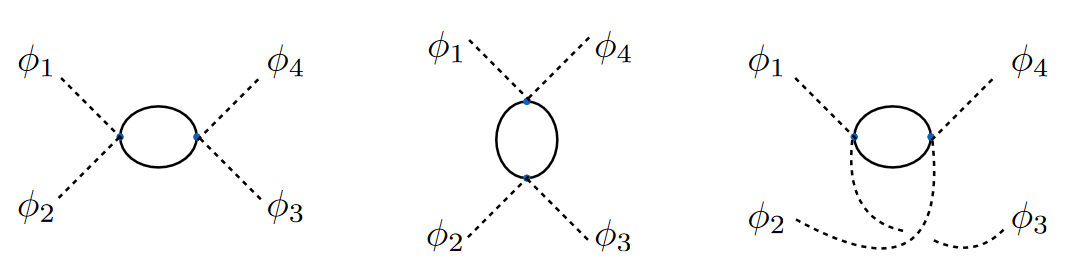
\includegraphics{2019/02/20190212_skinnerquartic.png}
\end{center}
which correspond to an amplitude
\begin{equation}
    \frac{\lambda^2}{2} \int^\Lambda \frac{d^4k}{(2\pi)^4}\frac{1}{k^2+m^2} \bkt{
        \frac{1}{(p_1+p_2+k)^2 +m^2}
        +\frac{1}{(p_1+p_4+k)^2+m^2}
        +\frac{1}{(p_1+p_3+k)^2+m^2}
    }.
\end{equation}
The overall factor of $1/2$ is a symmetry factor since the two internal lines are identical and can be exchanged, and the propagators can be read off by conservation of momentum at each vertex (taking all external momenta to be flowing in). We see that this integral goes as $d^4k/k^4$, so we expect a $\log\Lambda$ divergence. More precisely, the large $k$ behavior (where we care about this divergence) will look like%
    \footnote{This integral isn't totally immediate. To evaluate this, rewrite $k^3 dk= \frac{1}{2}k^2 d(k^2)$. Next, divide through in the numerator and denominator by $m^4$ to get
    \begin{equation*}
        \frac{1}{2}\int_0^\Lambda \frac{(k^2/m^2) d(k^2/m^2)}{(k^2/m^2) +1)^2}=\frac{1}{2}\int_0^{\Lambda^2/m^2} \frac{u\,du}{(u+1)^2}.
    \end{equation*}
    Finally, to evaluate the $u$ integral, just integrate by parts. Some similar integrals like $\int \frac{u\, du}{1+u}$ are amenable to a simple rewriting as $\frac{u}{1+u}=1-\frac{1}{1+u}$, but in general you'll want to integrate by parts:
    \begin{equation*}
        \int_0^{\Lambda^2/m^2} u\frac{du}{(1+u)^2}= -\left.\frac{u}{1+u}\right\rvert_0^{\Lambda^2/m^2} -\int \paren{-\frac{1}{1+u}}du=-\left.\frac{u}{1+u}\right\rvert_0^{\Lambda^2/m^2} +\left.\log(1+u)\right\rvert_0^{\Lambda^2/m^2}=\log\paren{1+\frac{\Lambda^2}{m^2}}-\frac{\Lambda^2}{\Lambda^2+m^2}.
    \end{equation*}
    
    }
\begin{align}
    \frac{3\lambda^2}{2} \int^\Lambda \frac{d^4k}{(2\pi)^4}\frac{1}{(k^2+m^2)^2} &= \frac{3\lambda^2}{16\pi^3} \int_0^\Lambda \frac{k^3 dk}{(k^2+m^2)^2}\\
    &= \frac{3\lambda^2}{32\pi^2} \int_0^{\Lambda^2/m^2} \frac{u\,du}{(1+u)^2}\\
    &= \frac{3\lambda^2}{32\pi^2} \bkt{
        \log\paren{1+\frac{\Lambda^2}{m^2}}-\frac{\Lambda^2}{\Lambda^2+m^2}\label{quarticdivergence}
    }.
\end{align}
This value is the shift in the $\lambda$ coupling before we introduce the $\delta \lambda$ counterterm.
If we then choose
\begin{equation}
    \delta \lambda =\frac{3\lambda^2}{32\pi^2} \bkt{\log \frac{\Lambda^2}{m^2}-1},
\end{equation}
we can then produce an effective coupling of 
\begin{equation}
    \lambda_{\text{eff}}=\lambda -\frac{3\lambda^2}{32\pi^2} \bkt{\log \paren{1+\frac{m^2}{\Lambda^2}}+\frac{m^2}{m^2+\Lambda^2}},
\end{equation}
which is finite as $\Lambda\to\infty$.%
    \footnote{
        This is just $\lambda$ plus the one-loop correction we computed to be \ref{quarticdivergence} plus our choice of $\delta \lambda$ (which is itself treated as a one-loop correction). In fact, we've neglected an overall minus sign in computing the one-loop correction. We should add a factor of $-i$ for the loop, and get rid of the $i$ as part of the overall momentum-conserving delta function which we've already dropped. Thus
        \begin{align*}
            \lambda_\text{eff}&=\lambda -\frac{3\lambda^2}{32\pi^2} \bkt{
                \log\paren{1+\frac{\Lambda^2}{m^2}}-\frac{\Lambda^2}{\Lambda^2+m^2}
            }
            +\frac{3\lambda^2}{32\pi^2} \bkt{\log \frac{\Lambda^2}{m^2}-1}\\
            &= \lambda -\frac{3\lambda^2}{32\pi^2} \bkt{\log \paren{1+\frac{m^2}{\Lambda^2}}+\frac{m^2}{m^2+\Lambda^2}}.
        \end{align*}
    }

For this next discussion, we'll need a trick due to Feynman:
\begin{equation}
    \int_0^1 \frac{dx}{\bkt{xA+(1-x)B}^2} =\frac{1}{B-1} \bkt{\frac{1}{xA+(1-x)B}}_0^1 = \frac{1}{AB}.
\end{equation}
We'll use this to rewrite products of denominators as these sorts of integrals, i.e. from right to left. Note that the integral can be put in a more manifestly symmetric form as
\begin{equation*}
    \int_0^1 dx \int_0^1 dy \frac{\delta(x+y-1)}{(xA+yB)^2}.
\end{equation*}

For our first diagram, let $p_{12}\equiv p_1 +p_2$. Then the propagators take the form
\begin{align*}
    \frac{1}{(p_{12}+k)^2+m^2}\frac{1}{k^2+m^2}&=\int_0^1 \frac{dx}{\bkt{x((p_{12}+k)^2+m^2)+(1-x)(k^2+m^2)}^2
    }\\
        &= \int_0^1 \frac{dx}{\bkt{(k+xp_{12})^2 +m^2 +x(1-x)p_{12}^2}^2}\\
        &= \int_0^1 \frac{dx}{\bkt{l^2+m^2+x(1-x)p_{12}^2}^2}
\end{align*}
where we have defined $l=k+x p_{12}.$
In the $\Lambda \to \infty$ limit, the shifted integration range $|k|\leq \Lambda \to |l|\leq \Lambda$ vanishes, so we can turn our $d^4k$ integral into a $d^4 l$ and write
\begin{align*}
    \int \frac{d^4ldx}
    {\bkt{l^2+m^2+x(1-x)p_{12}^2}^2}
    &= S_4 \int_0^1 dx \int_0^\Lambda \frac{l^3 dl}
    {\bkt{l^2+m^2+x(1-x)p_{12}^2}^2}\\
    &= \pi \int_0^1 dx \set*{ \log \bkt{
        \frac{\Lambda^2 +m^2+x(1-x)p_{12}^2}{m^2+m^2+x(1-x)p_{12}^2}
    }
    +\frac{m^2+x(1-x)p_{12}^2}{\Lambda^2+m^2+x(1-x)p_{12}^2}
    -1
    }
\end{align*}
after a change of variables and an integration by parts. Note that this term with the $1/\Lambda^2$ goes to zero as $\Lambda\to\infty$. Let's notice that all three diagrams are related by the Mandelstam variables 
\begin{equation}
    s=-(p_1+p_2)^2,t=-(p_1+p_4)^2,u=-(p_1+p_3)^2,
\end{equation}
so that the sum of our three diagrams is then
\begin{equation}
    \frac{\lambda^2}{32\pi^2}\int_0^1 dx \set*{ \log \paren{\frac{\Lambda^2}{m^2-x(1-x)s}} 
    + \log \paren{\frac{\Lambda^2} {m^2-x(1-x)t}}
    + \log \paren{\frac{\Lambda^2} {m^2-x(1-x)u}}
    -3
    }.
\end{equation}
The coefficient of $\tilde \phi^4$ in the effective action $\Gamma(\tilde \phi)$ (i.e. $\tilde \phi$ in momentum space) is
\begin{equation}
    \lambda+\delta \lambda -\frac{\lambda^2}{32\pi^2} \int d \set{\ldots}
\end{equation}
with $\delta \lambda$ from above, and replacing $(m^2,\lambda)\mapsto (m_{\text{phys}}^2,\lambda_{\text{eff}})$.
We find that 
\begin{equation}
    \lambda_{\text{eff}}+\frac{\lambda_{\text{eff}}^2}{32\pi^2} \int_0^1 dx \set*{ \log \bkt{1-\frac{x(1-x)s}{m_{\text{phys}}^2}}
    +\log \bkt{1-\frac{x(1-x)t}{m_{\text{phys}}^2}}
    +\log \bkt{1-\frac{x(1-x)u}{m_{\text{phys}}^2}}
    }
\end{equation}
is finite-- no more counterterms are necessary after $\delta m^2$ and $\delta \lambda$. Our capacity to regulate these terms depends on the idea of operators being relevant, irrelevant, or marginal (depending on their mass dimension as compared to the dimension of spacetime).
\end{document}